
%%%%%%%%%%%%%%%%%%%%%%%%%%%%%%%%%%%%%%%%%%%%%%%%%%%%%%%%%%%%%%%%%%%%%%%%%%%%%%%%%%%%%%%
%%%%%%%%%%%%%%%%%%%%%%%%%%%%%%%%%%%%%%%%%%%%%%%%%%%%%%%%%%%%%%%%%%%%%%%%%%%%%%%%%%%%%%%
% 
% This top part of the document is called the 'preamble'.  Modify it with caution!
%
% The real document starts below where it says 'The main document starts here'.

\documentclass[12pt]{article}

\usepackage{amssymb,amsmath,amsthm}
\usepackage[top=1in, bottom=1in, left=1.25in, right=1.25in]{geometry}
\usepackage{fancyhdr}
\usepackage{enumerate}
\usepackage{listings}
\usepackage{graphicx}
\usepackage{float}

\usepackage{mwe}
\usepackage{caption}
\usepackage{subcaption}
% Comment the following line to use TeX's default font of Computer Modern.
\usepackage{times,txfonts}



\makeatletter
\renewcommand*\env@matrix[1][*\c@MaxMatrixCols c]{%
  \hskip -\arraycolsep
  \let\@ifnextchar\new@ifnextchar
  \array{#1}}
\makeatother

\newtheoremstyle{homework}% name of the style to be used
  {18pt}% measure of space to leave above the theorem. E.g.: 3pt
  {12pt}% measure of space to leave below the theorem. E.g.: 3pt
  {}% name of font to use in the body of the theorem
  {}% measure of space to indent
  {\bfseries}% name of head font
  {:}% punctuation between head and body
  {2ex}% space after theorem head; " " = normal interword space
  {}% Manually specify head
\theoremstyle{homework} 

% Set up an Exercise environment and a Solution label.
\newtheorem*{exercisecore}{Exercise \@currentlabel}
\newenvironment{exercise}[1]
{\def\@currentlabel{#1}\exercisecore}
{\endexercisecore}

\newcommand{\localhead}[1]{\par\smallskip\noindent\textbf{#1}\nobreak\\}%
\newcommand\solution{\localhead{Solution:}}

%%%%%%%%%%%%%%%%%%%%%%%%%%%%%%%%%%%%%%%%%%%%%%%%%%%%%%%%%%%%%%%%%%%%%%%%
%
% Stuff for getting the name/document date/title across the header
\makeatletter
\RequirePackage{fancyhdr}
\pagestyle{fancy}
\fancyfoot[C]{\ifnum \value{page} > 1\relax\thepage\fi}
\fancyhead[L]{\ifx\@doclabel\@empty\else\@doclabel\fi}
\fancyhead[C]{\ifx\@docdate\@empty\else\@docdate\fi}
\fancyhead[R]{\ifx\@docauthor\@empty\else\@docauthor\fi}
\headheight 15pt

\def\doclabel#1{\gdef\@doclabel{#1}}
\doclabel{Use {\tt\textbackslash doclabel\{MY LABEL\}}.}
\def\docdate#1{\gdef\@docdate{#1}}
\docdate{Use {\tt\textbackslash docdate\{MY DATE\}}.}
\def\docauthor#1{\gdef\@docauthor{#1}}
\docauthor{Use {\tt\textbackslash docauthor\{MY NAME\}}.}
\makeatother

% Shortcuts for blackboard bold number sets (reals, integers, etc.)
\newcommand{\Reals}{\ensuremath{\mathbb R}}
\newcommand{\Nats}{\ensuremath{\mathbb N}}
\newcommand{\Ints}{\ensuremath{\mathbb Z}}
\newcommand{\Rats}{\ensuremath{\mathbb Q}}
\newcommand{\Cplx}{\ensuremath{\mathbb C}}
%% Some equivalents that some people may prefer.
\let\RR\Reals
\let\NN\Nats
\let\II\Ints
\let\CC\Cplx

%%%%%%%%%%%%%%%%%%%%%%%%%%%%%%%%%%%%%%%%%%%%%%%%%%%%%%%%%%%%%%%%%%%%%%%%%%%%%%%%%%%%%%%
%%%%%%%%%%%%%%%%%%%%%%%%%%%%%%%%%%%%%%%%%%%%%%%%%%%%%%%%%%%%%%%%%%%%%%%%%%%%%%%%%%%%%%%
% 
% The main document start here.

% The following commands set up the material that appears in the header.
\doclabel{STAT 401: Homework 8}
\docauthor{Stefano Fochesatto}
\docdate{\today}


%\begin{figure}[H]
%  \begin{center}
%  \caption{}
%  \includegraphics[\textwidth]{}
%  \end{center}
%\end{figure}

% \textbf{Code:}
% \begin{center}
% \lstinputlisting{}
% \end{center} 



\begin{document}

\begin{exercise}{1} Do problem 9.8. Draw residual plots for the mean function described in Problem 8.3.4
  for the California water data, and comment on your results. Test for curvature as a function of fitted values.\\
  \solution Recall that problem 8.3.2 described the following model, 
  \begin{equation*}
    \log(BSAAM) \thicksim \log(APMAM)+\log(APSAB)+\log(APSLAKE)+\log(OPBPC)+\log(OPRC)+\log(OPSLAKE)
  \end{equation*}
  Creating the model in r, and calling the residualplots() we get the following figure. We can see that the residual plots 
  for each first order predictor do not exhibit significant curvature. Each plot looks fairly random, and when we consider the tests on the second order predictors 
  that are produced by residualplots(), at an $\alpha = .05$ significance level we get that our residual plots show little curvature. 
  \begin{figure}[H]
    \begin{center}
    \caption{Residual Plots for 8.3.2 model.}
    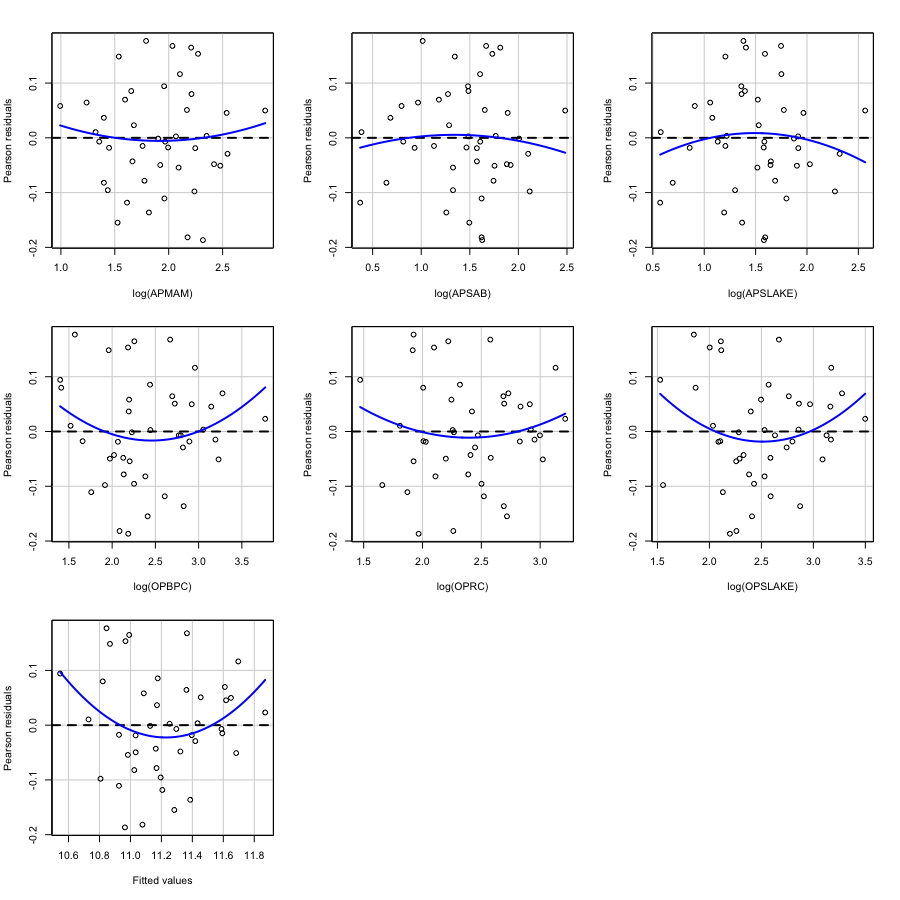
\includegraphics[width = .94\textwidth]{Rplot.png}
  \end{center}
\end{figure}
\textbf{Code:}
\begin{center}
\lstinputlisting{r1.txt}
\end{center} 

\end{exercise}
\newpage



\begin{exercise}{2} Do problem 9.3, and skip part 9.3.3. This example compares in=field ultrasonic measurements of depths of defects, Field, in the 
  Alaska oil pipeline with measurements of the same defects in a laboratory, Lab. the lab measurements were done in six different batches, in the variable Batch. The 
  goals is to decide if the field measurement san be used to predict the more accurate lab measurements. The lab measurement is the response variable and the field measurement 
  is the predictor variable. The data are from National institute of Science and Technology.\\
  \begin{enumerate}
    \item[9.3.1] Draw the scatterplot of Lab vs Field, and comment on the applicability of a simple linear regression model.\\
    \solution  Using r we get the following scatterplot(code is in next part). Here a simple linear regression would likely do a bad job at explaining the 
    relationship between Lab and Field data. In an early module we discussed how when a scatterplot has a fan shape that is an 
    indication of non-constant variance of an SLR model. We can see that as our lab results grow in size so does the spread of the data resulting 
    in the fan shape that we discussed previously. 
    \begin{figure}[H]
      \begin{center}
      \caption{Lab vs Field Scatterplot}
      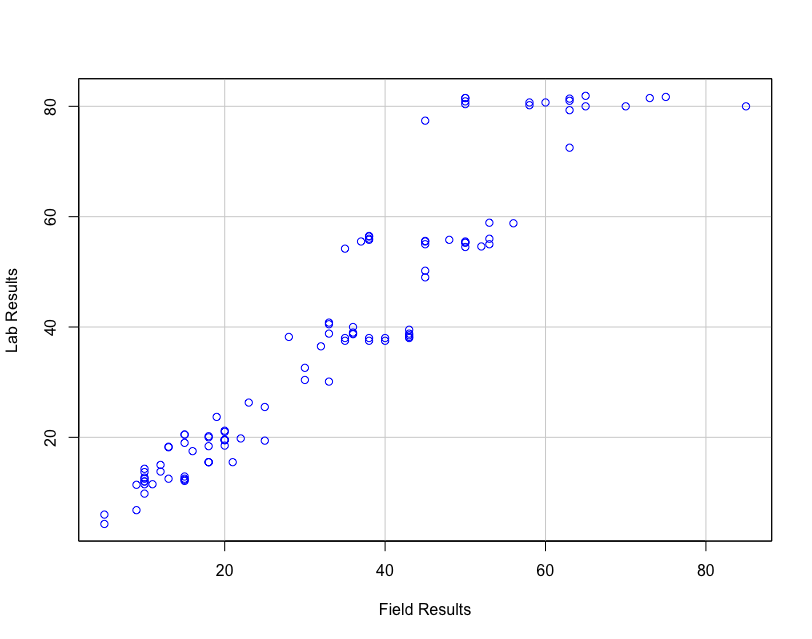
\includegraphics[width = .94\textwidth]{Rplot01.png}
    \end{center}
  \end{figure}
  \newpage




    \item[9.3.2] Fit the simple regression model, get the residual plot, and summarize. Explain why the plot suggests non-constant variance and 
    provide a test for non-constant variance.\\
    \solution Fitting the SLR model and producing the residual plot in r we get the following. The residual plot shows a left to right fanning pattern (like $'<'$)
    which suggests that we are dealing with a non-constant variance. With a p-value of 5.3499e-08 the Bruesch-Pagan test confirms our idea that we are dealing with non-constant variance. 

    \begin{figure}[H]
      \begin{center}
      \caption{Residual Plots for Pipeline SLR}
      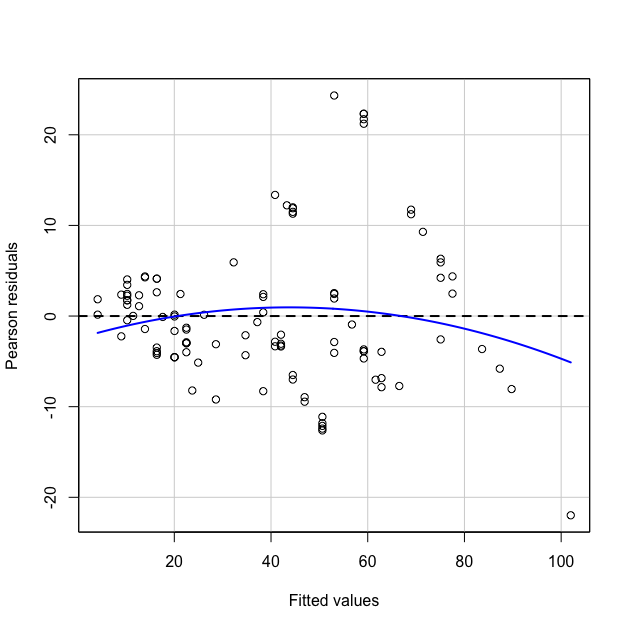
\includegraphics[width = .94\textwidth]{Rplot02.png}
    \end{center}
  \end{figure}
  \textbf{Code:}
  \begin{center}
  \lstinputlisting{r2.txt}
  \end{center} 
  \end{enumerate}
\end{exercise}
\newpage



\begin{exercise}{3} Using the data and model fit in problem 9.8, do the following, 
  \begin{enumerate}
    \item Perform a test for outliers and interpret the test's results. \\
    \solution Using the outlierTest() function and computing the t-statistic for all studentized residuals in r 
    we get that there are no outliers even if we adjust our significance by using the Bonferroni p-value, \\
    \textbf{Code:}
    \begin{center}
    \lstinputlisting[basicstyle = \footnotesize]{r3.txt}
    \end{center} 
    \newpage

    \item Determine whether any observations are highly influential, as measured by Cook's D.\\
    \solution Using the cooks.distance() function in r we can find which observations have high influence.
    Since there are conflicting practices for determining the significance of the Cook's D benchmark we will consider both the 
    greater than 1 and greater than 4/n criteria. From r, we got that with the 4/n criteria there are 5 highly influential observations
    that seem to be spread out evenly throughout the data. With the greater than 1 criteria we get that there are no influential observations. 
    \begin{figure}[H]
      \begin{center}
      \caption{Plot of Cook's D Values, With 4/n Criteria}
      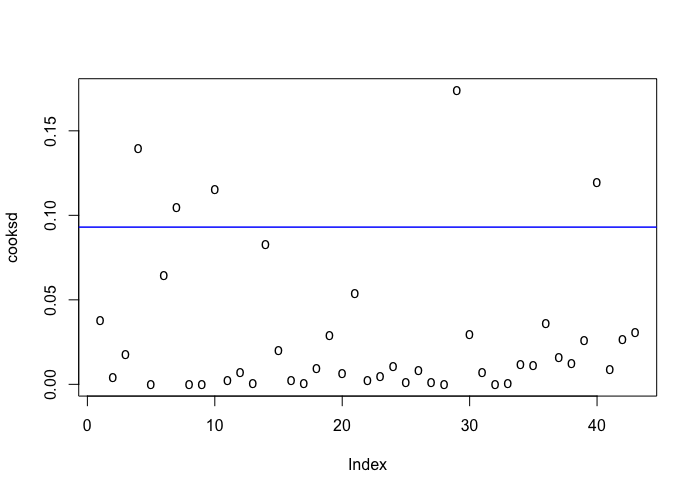
\includegraphics[width = .94\textwidth]{Rplot03.png}
    \end{center}
  \end{figure}
  \textbf{Code:}
  \begin{center}
  \lstinputlisting[basicstyle = \footnotesize]{r4.txt}
  \end{center} 
  \newpage



    \item Perform a Durbin-Watson test of independence in the residuals and interpret the test's result.\\
    \solution Performing the Durbin-Watson test in r, we get a p-value of 0.034. On the $\alpha = .05$ we reject the null hypothesis 
    and concluded that there does exists some autocorrelation among the residuals of the model. With a p-value so close to our significance 
    threshold we might be able to get away with using the model, however this results warrants further analysis. We could try to refit the model 
    with different(less) predictors or we could try some transformations on the data. \\
    \textbf{Code:}
    \begin{center}
    \lstinputlisting[basicstyle = \footnotesize]{R5.TXT}
    \end{center} 
    \newpage
    




    \item Obtain a normal probability plot and perform a a Shapiro Wilk test of normality in the residuals. Interpret the test's
    results and the plot. \\
    \solution Producing the normal probability plot and performing the Shapiro-Wilk test we get that the residuals are normally distributed. 
    The normal probability plot shows some group of residuals below the fitted line in the beginning and above the fitted line at the end. This suggests
    that the probability distribution for our residuals had larger tails than that of a normal or t-distributions. With a p-value of 0.6659, we reject the null and the 
    Shapiro-Wilk test tells us that this difference is insignificant on the $\alpha = .05$ level. 
    \begin{figure}[H]
      \begin{center}
      \caption{Normal Probability Plot for WaterModel Residuals}
      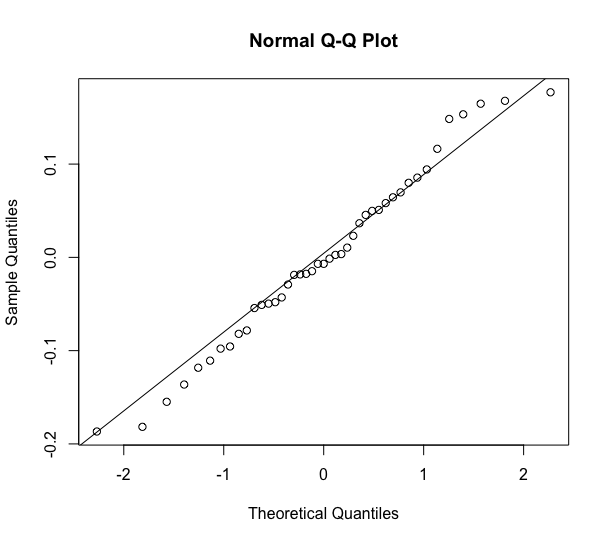
\includegraphics[width = .80\textwidth]{Rplot04.png}
    \end{center}
  \end{figure}
  \textbf{Code:}
  \begin{center}
  \lstinputlisting[basicstyle = \footnotesize]{r6.txt}
  \end{center} 
  \newpage

    \item Perform a test for non-constant variance in the residuals vs. fitted values plot. Interpret the test's results. \\
    \solution Using the residualPlots() command we can obtain the residual plots for each predictor, as well as the fitted values of 
    the model. We also get the p-values for the significance of second order predictors, as well as Tukey's test for non-constant variance. 
    Tukey's test shows us that with a p-value of 0.06597, on the $\alpha = .05$ level the residuals demonstrate constant variance.
    \begin{figure}[H]
      \begin{center}
      \caption{Residual Plots for WaterMode}
      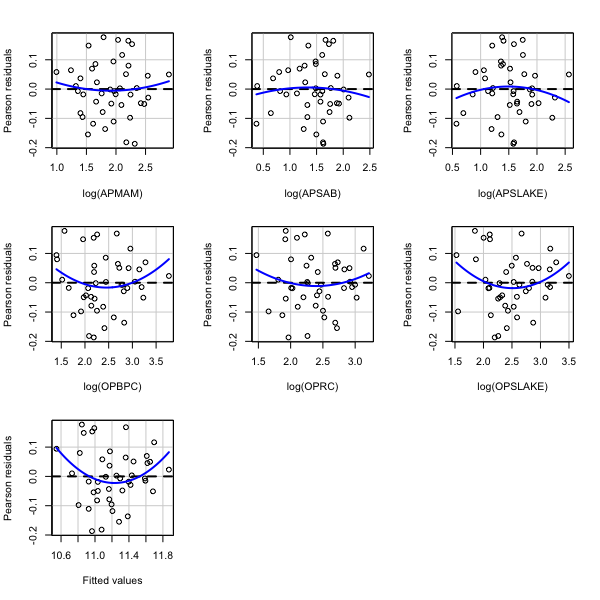
\includegraphics[width = .80\textwidth]{Rplot05.png}
    \end{center}
  \end{figure}
  \textbf{Code:}
  \begin{center}
  \lstinputlisting[basicstyle = \footnotesize]{r7.txt}
  \end{center} 
  \newpage



    \item Summarize all your finding from the diagnostics of this model and make recommendations about whether this model's results should be 
    trusted. \\
    \solution Of the tests that we performed we found there to be several influence points using the 4/n criteria for the Cook's D test. 
    We also found, from the Durbin-Watson test that there does exists some autocorrelation in the residuals of the model. In that problem we 
    suggested that we could try transforming the data or fitting the data with different predictors. In any case, I would encourage further analysis 
    before trusting this model, maybe through PCA we can test out different predictors and transformations to get a better model. 
  \end{enumerate}
  
\end{exercise}



\end{document}





















